% !Mode:: "TeX:UTF-8"
%% 请使用 XeLaTeX 编译本文.
% \documentclass{WHUBachelor}% 选项 forprint: 交付打印时添加, 避免彩色链接字迹打印偏淡. 即使用下一行:
\documentclass[forprint]{WHUBachelor}
%---------------------这里添加所需的package--------------------------------
\usepackage{url}

%--------------------------------------------------------------------------
\makeatletter
\def\BState{\State\hskip-\ALG@thistlm}
\makeatother
\begin{document}
%-----------------------------------------------------------------------------

%%%%%%% 下面的内容, 据实填空.

\Ccoursename{XXX课程} %课程名称
\title{ ~\LaTeX~ 模板及使用教程\\Introduction of ~\LaTeX~ Template} %实验名称 换行请使用\\
\author{} % 学生姓名
\Csupervisor{XXXX \quad 教授} %指导教师一姓名、职称

% 默认不显示指导教师二,需要时可在WHUBachelor.cls 80+行处将"关闭第二指导教师显示"下一行的注释解除
\CsupervisorAnother{无} %指导教师二姓名、职称 

\CstudentNum{XXXX} %学号
\Cmajor{XXXX} % 专业名称
\date{二〇一九年六月} % 日期

%-----------------------------------------------------------------------------

\pdfbookmark[0]{封面}{title}         % 封面页加到 pdf 书签
\maketitle
\frontmatter
\pagenumbering{Roman}              % 正文之前的页码用大写罗马字母编号.2019.6.16:更新 正文之前的页码隐藏,无需显示
%-----------------------------------------------------------------------------
% !Mode:: "TeX:UTF-8"

%%% 此部分需要自行填写: 中文摘要及关键词 

%%% 郑重声明部分无需改动

%%%---- 郑重声明 (无需改动)------------------------------------%
\newpage
\thispagestyle{empty}
\vspace*{20pt}
\begin{center}{\ziju{0.8}\pmb{\songti\zihao{2} 郑重声明}}\end{center}
\par\vspace*{30pt}
\renewcommand{\baselinestretch}{2}

{\zihao{4}%

本人呈交的设计报告,是在指导老师的指导下,独立进行实验工作所取得的成果,
所有数据、图片资料真实可靠。 尽我所知,除文中已经注明引用的内容外,
本设计报告不包含他人享有著作权的内容。
对本设计报告做出贡献的其他个人和集体,
均已在文中以明确的方式标明。本设计报告的知识产权归属于培养单位。\\[2cm]

\hspace*{1cm}本人签名: $\underline{\hspace{3.5cm}}$
\hspace{2cm}日期: $\underline{\hspace{3.5cm}}$\hfill\par}
%------------------------------------------------------------------------------
\baselineskip=23pt  % 正文行距为 23 磅
%------------------------------------------------------------------------------





%%======摘要===========================%
\begin{cnabstract}
\thispagestyle{empty}

本文使用武汉大学计算机学院实验报告的~\LaTeX~模板,并介绍~\LaTeX~和模板的使用。

\begin{itemize}
    \item 本项目仓库地址:\url{https://github.com/Nagico/WHUExperiment}
    \item 参考repo:
    \begin{enumerate}
        \item \url{https://github.com/whutug/whu-thesis}
        \item \url{https://github.com/xiaoxinganling/WHUExperiment}
    \end{enumerate}
\end{itemize}

欢迎进入仓库中给开发者一个免费的star\textasciitilde


\end{cnabstract}
\par
\vspace*{2em}


%%%%--  关键词 -----------------------------------------%%%%%%%%
%%%%-- 注意: 每个关键词之间用“;”分开,最后一个关键词不打标点符号
\cnkeywords{实验报告; \LaTeX{}; 模板   }



    % 加入摘要, 申明.
%==========================把目录加入到书签==============================%%%%%%


\tableofcontents
\thispagestyle{empty}				%不显示罗马数字 ——zmx更新于2019.06.18
\addtocontents{toc}{\protect\thispagestyle{empty}}




\mainmatter %% 以下是正文
%%%%%%%%%%%%%%%%%%%%%%%%%%%--------main matter-------%%%%%%%%%%%%%%%%%%%%%%%%%%%%%%%%%%%%
\pagestyle{plain}%plain
%\cfoot{\thepage{\zihao{5}\bf\usefonttimes}}
%\renewcommand{\baselinestretch}{1.6}
%\setlength{\baselineskip}{23pt}
\baselineskip=23pt  % 正文行距为 23 磅

%此处书写正文-------------------------------------------------------------------------------------

\chapter{~\LaTeX~ 介绍}

~\LaTeX~是一种基于Tex的排版系统,它不像Word软件编写文件一样所见即所得,而是用一定的语法或者标记符号来组织内容。~\LaTeX~在学术写作中被广泛使用,特别是像数学和计算机这样的学科。~\LaTeX~可以让你忘记格式,而专注于内容。

有人可能会问我们已经有Word了,用起来也很方便啊,为什么还要用~\LaTeX~这种还有些技术门槛的工具呢?其实在学术写作中,我们往往会对内容不停地改来改去,特别是如果还插入了图片的话,每次修改都可能需要重新排版。而~\LaTeX~可以让你不用担心这些,任何时候都能帮你输出高质量的排版。

\section{~\LaTeX~优点}

经常有人喜欢对比 ~\LaTeX~ 和以 Word 为代表的“所见即所得”(What You See Is What You Get)字处理工具。这种对比是没有意义的,因为 TEX 是一个排版引擎,~\LaTeX~ 是其封装,而 Word 是字处理工具。二者的设计目标不一致,也各自有自己的适用范围。 不过,这里仍旧总结 ~\LaTeX~ 的一些优点:

%\cite{axiangBaYiBaLaTeXHeWordXiangBiQiYouQueDian2021}

\begin{itemize}
    \item 具有专业的排版输出能力
    \item 具有方便而强大的数学公式排版能力
    \item 绝大多数时候,用户只需专注于一些组织文档结构的基础命令,无需(或很少)操心文档 的版面设计
    \item 很容易生成复杂的专业排版元素,如脚注、交叉引用、参考文献、目录等
    \item 强大的可扩展性,世界各地的人开发了数以千计的 ~\LaTeX~ 宏包用于补充和扩展 ~\LaTeX~ 的功能
    \item 能够促使用户写出结构良好的文档,而这也是 ~\LaTeX~ 存在的初衷
\end{itemize}

\section{~\LaTeX~缺点}

同时不可否认的是,~\LaTeX~的使用需要一定的学习门槛,同时在使用过程中存在以下缺点:

\begin{itemize}
    \item 不容易排查错误。~\LaTeX~ 作为一个依靠编写代码工作的排版工具,其使用的宏语言比 C++ 或 Python 等程序设计语言在错误排查方面困难得多。它虽然能够提示错误,但不提供调试的机制,有时错误提示还很难理解。
    \item 不容易定制样式。~\LaTeX~ 提供了一个基本上良好的样式,为了让用户不去关注样式而专注于文档结构。但如果想要改进 ~\LaTeX~ 生成的文档样式则是十分困难,需要系统的学习~\LaTeX~排版。
    \item 相比“所见即所得”的模式有一些不便,为了查看生成文档的效果,用户总要不停地编译。
\end{itemize}


\chapter{~\LaTeX~的安装}

~\LaTeX~的使用需要安装相关的软件,目前主要使用的有两种方式进行~\LaTeX~编辑:
\begin{itemize}
  \item 在线编辑器(Overleaf、TeXPage)
  \item 本地编辑器(VSCode+插件、TeXShop)
\end{itemize}

个人推荐使用Overleaf进行编辑,无需安装本地编译环境,同时还可以进行多人协同操作。但使用在线编辑器的缺点就是必须连接网络。

\section{Overleaf的使用}

进入到Overleaf首页:\url{https://www.overleaf.com},点击右上角Register注册新账户。登录成功后如图\ref{fig:2-overlead-home}所示,会进入到项目界面。

\begin{figure}[htb]
  \centering
  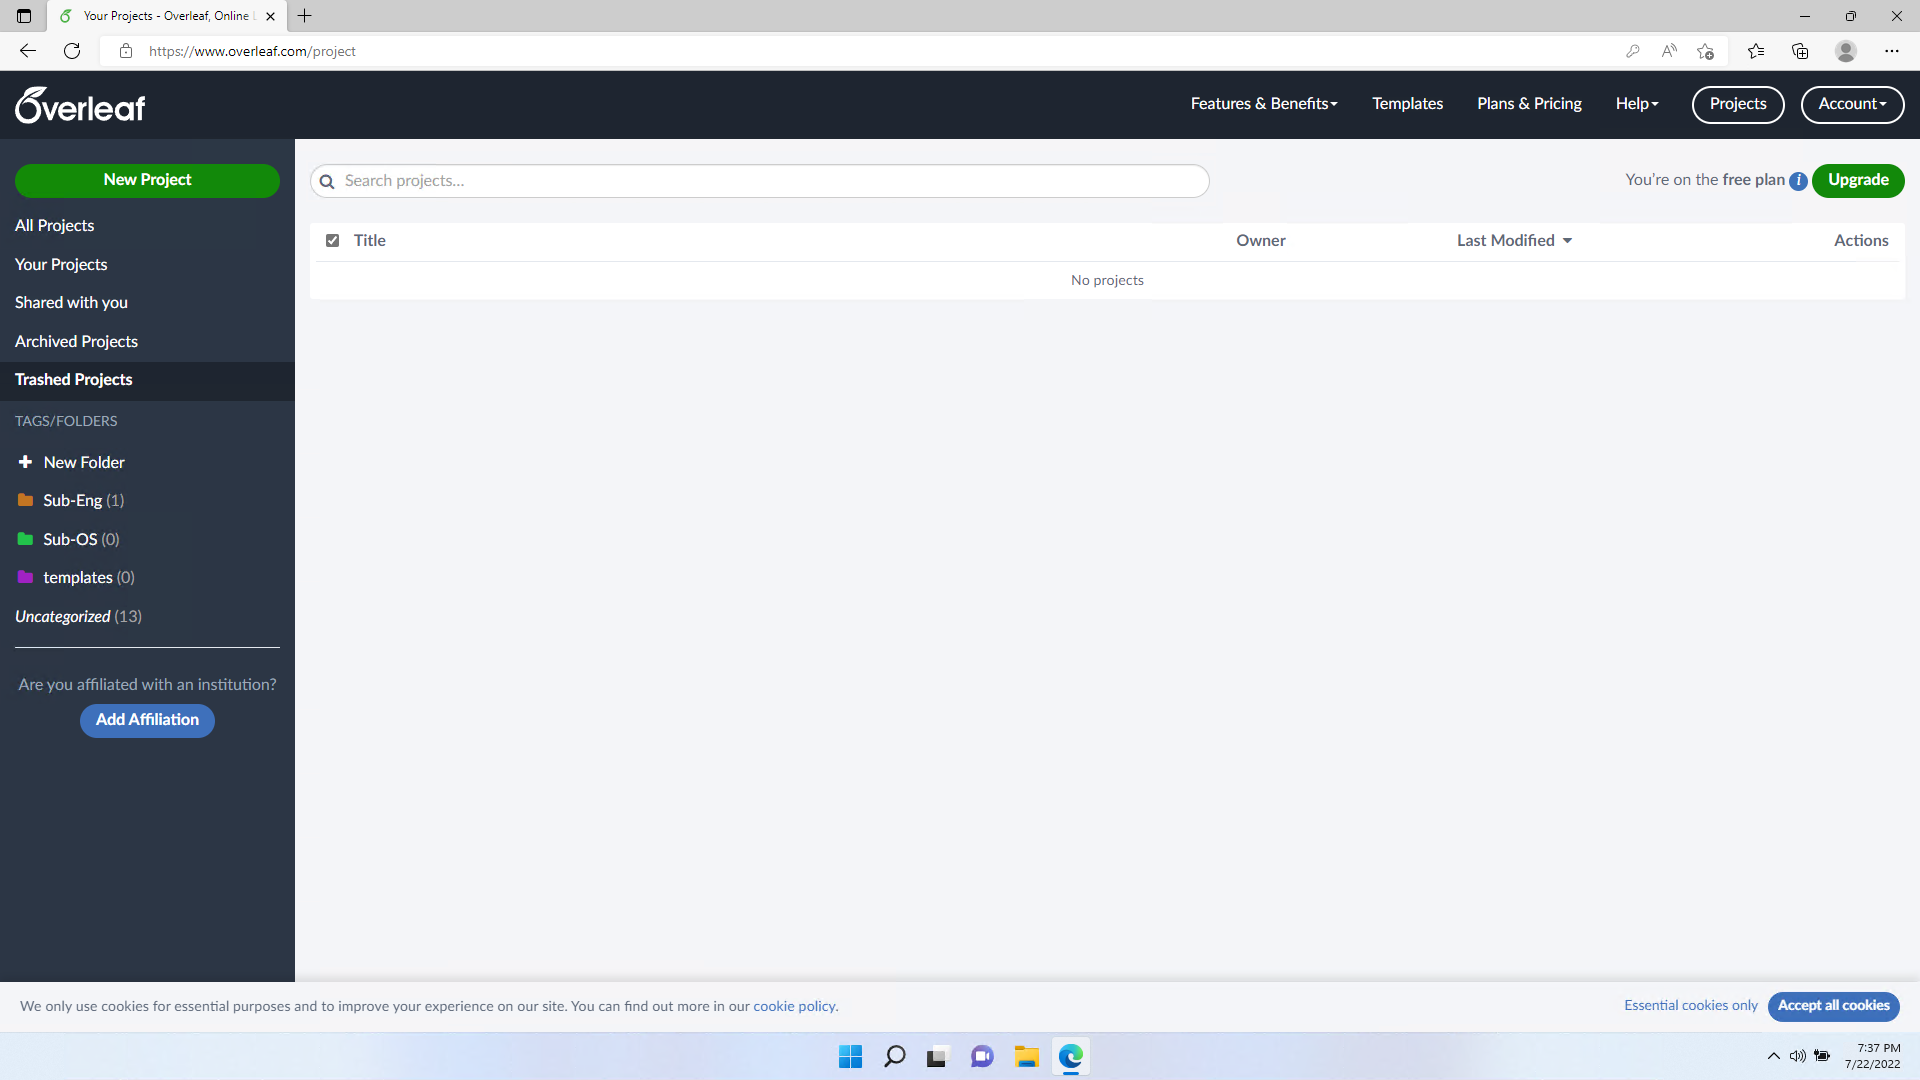
\includegraphics[width=0.9\textwidth]{figures/chapter2/overleaf-home.png}
  \caption{Overleaf项目页面}
  \label{fig:2-overlead-home}
\end{figure}

此时你需要将使用的模板下载至本地。以此项目为例,进入\url{https://github.com/Nagico/WHUExperiment},点击Download ZIP即可将模板下载到本地。该模板同时也一同放至本文档旁,可以直接使用,但仍建议从Github上下载最新版本的模板。

\begin{figure}[htb]
    \centering
    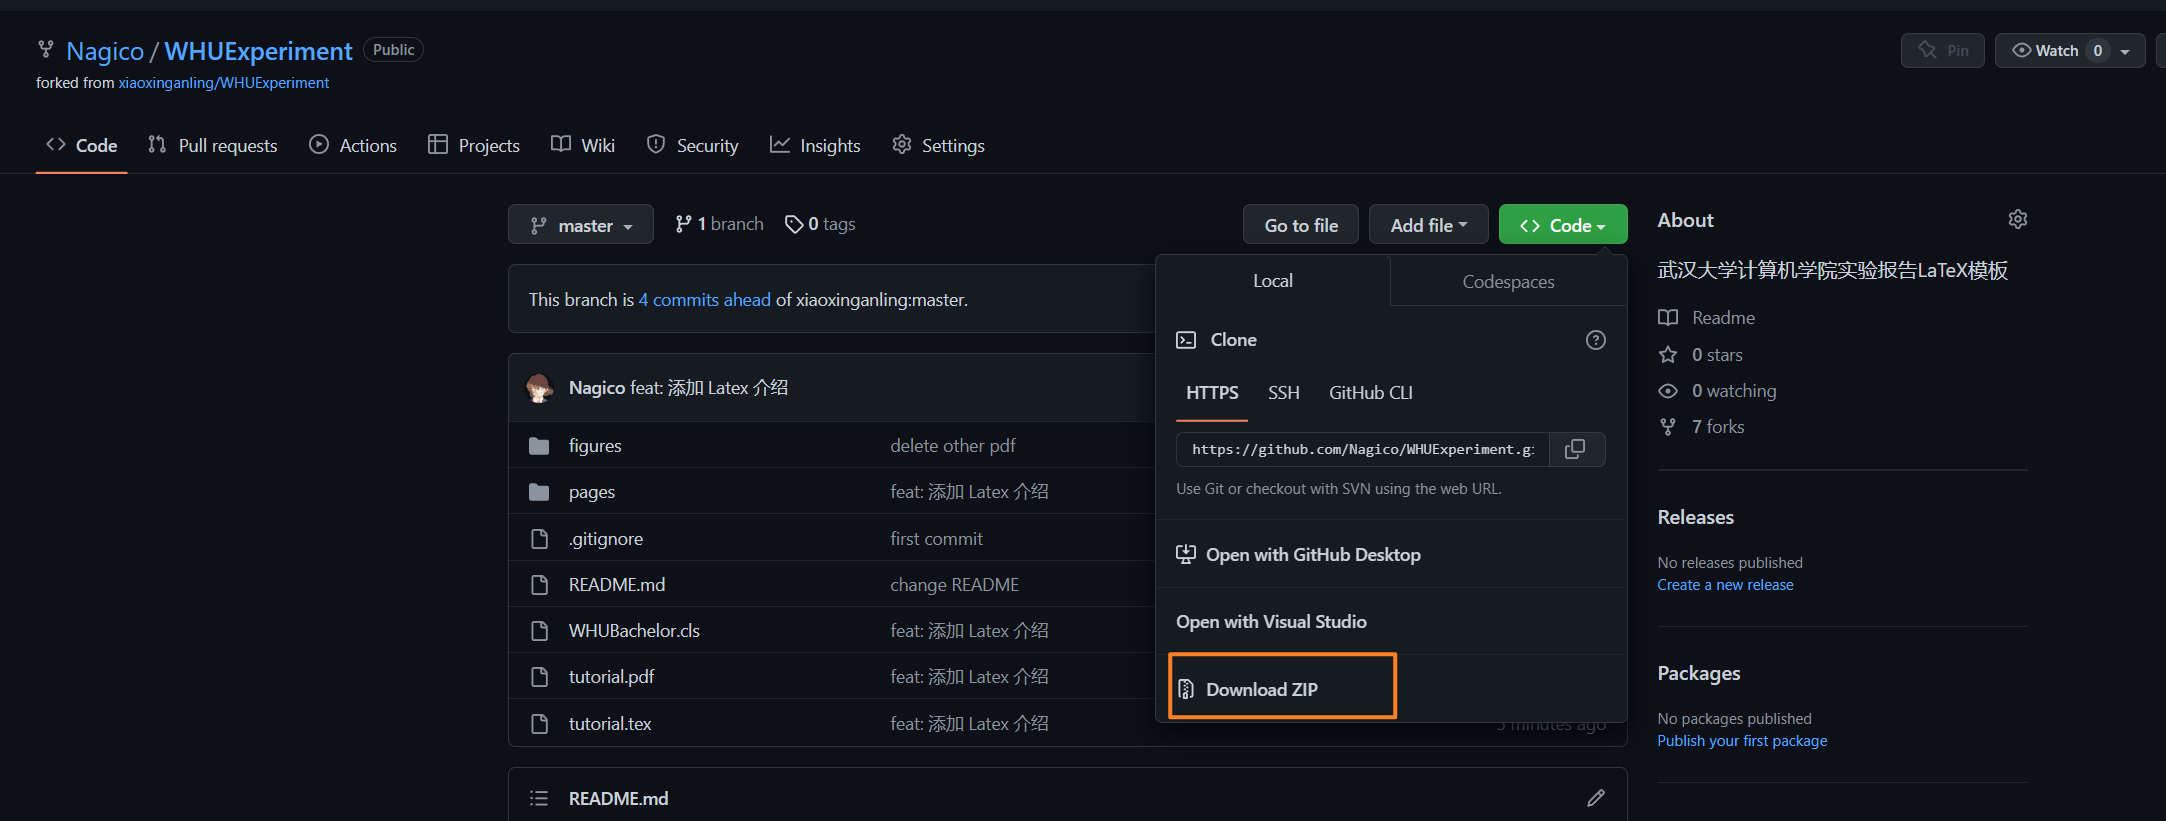
\includegraphics[width=0.95\textwidth]{figures/chapter2/download-repo.png}
    \caption{下载模板}
    \label{fig:2-github-download}
\end{figure}

在Overleaf页面点击左侧的New Project,选择Upload Project,将下载的ZIP文件上传,即可将模板导入至Overleaf。

\begin{figure}[htb]
  \centering
  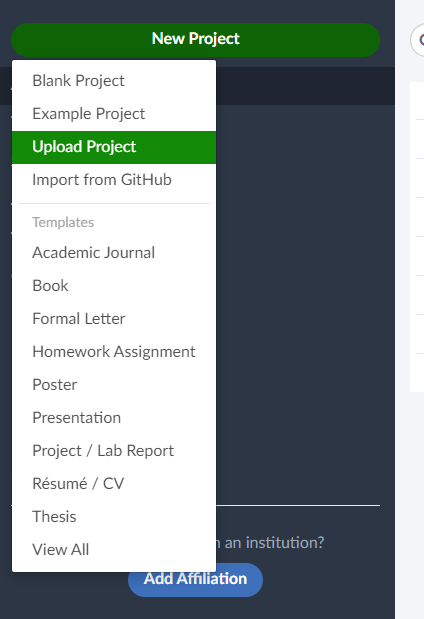
\includegraphics[width=0.3\textwidth]{figures/chapter2/upload-project.png}
  \caption{导入模板}
  \label{fig:2-upload-project}
\end{figure}

导入后会自动跳转到编辑界面,需要点击左上角的Menu进入设置界面,将Compiler修改为XeLatex以支持中文(图\ref{fig:2-compiler})。

\begin{figure}[H]
  \centering
  \begin{subfigure}{0.55\textwidth}
    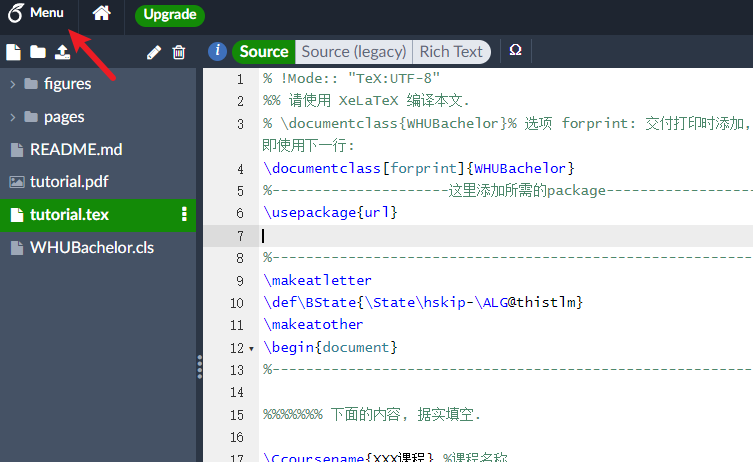
\includegraphics[width=\linewidth]{figures/chapter2/menu.png}
    \caption{Menu按钮}
    \label{fig:2-menu}
  \end{subfigure}\qquad
  \begin{subfigure}{0.3\textwidth}
    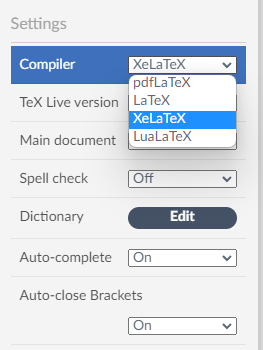
\includegraphics[width=\linewidth]{figures/chapter2/xelatex.png}
    \caption{选择Compiler}
    \label{fig:2-compiler}
  \end{subfigure}
  \caption{配置~\LaTeX~}
  \label{fig:2-latex-conf}
\end{figure}

修改成功后点击Recompile重新编辑,即可正常使用。你可以在左侧进行项目文件的管理,后续所需的图片可以在相应文件夹处右键,选择Upload上传。

\begin{figure}[htb]
  \centering
  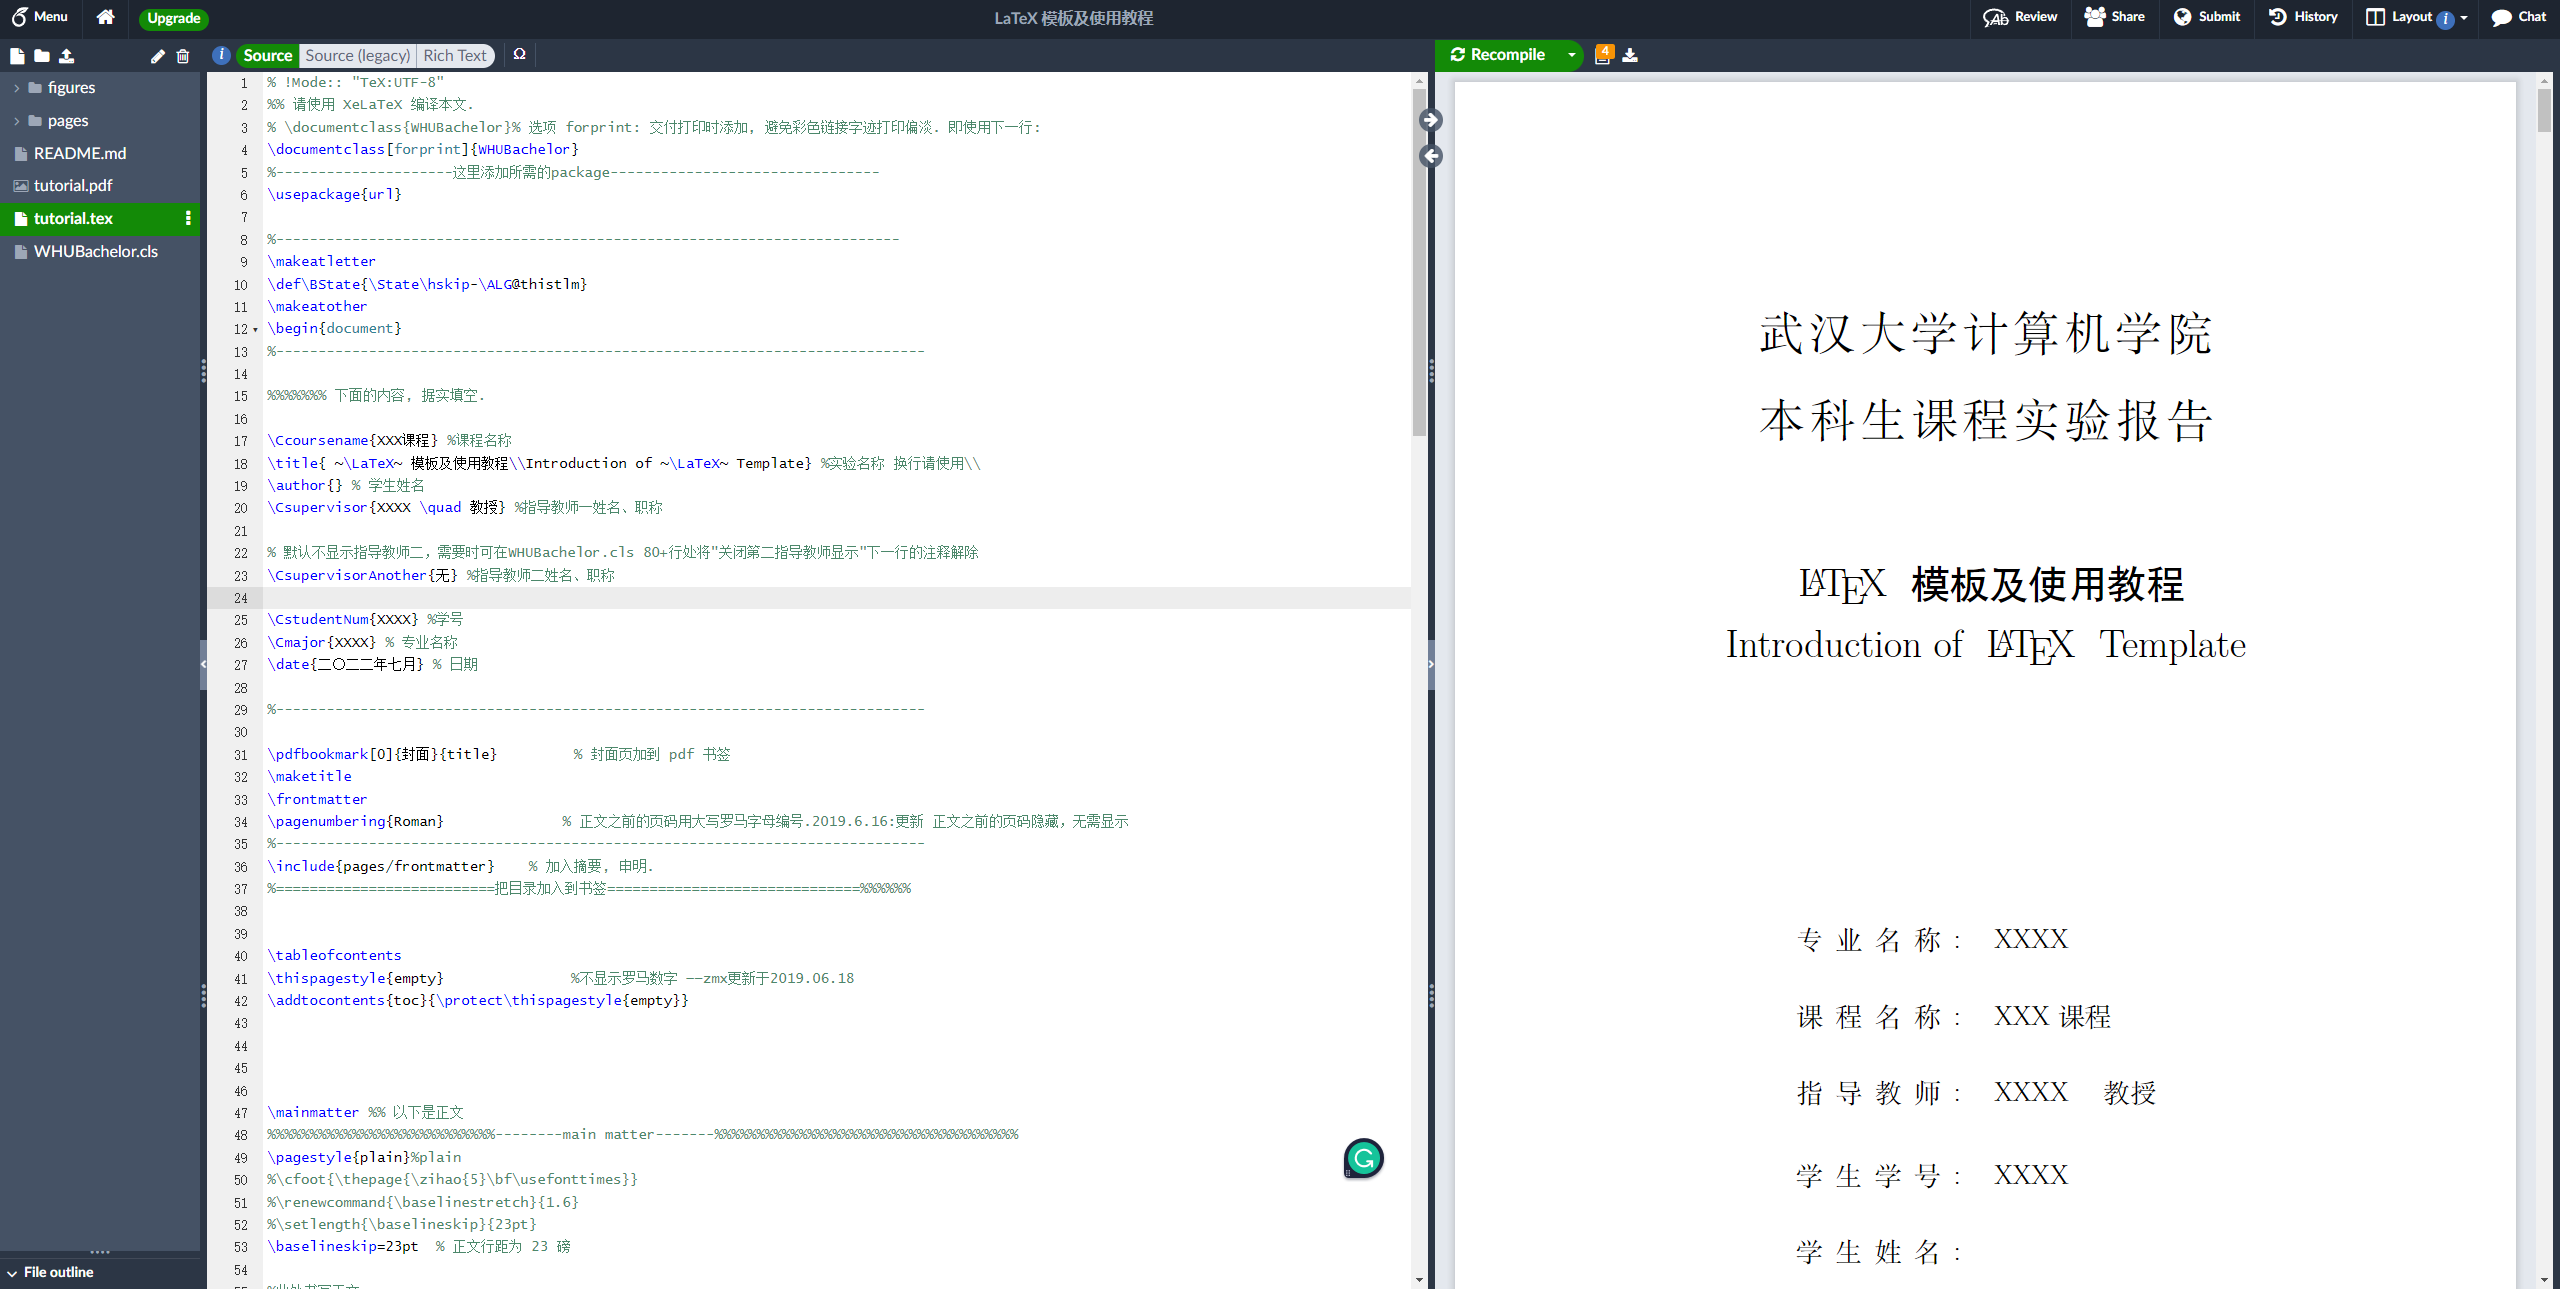
\includegraphics[width=0.95\textwidth]{figures/chapter2/overleaf-edit.png}
  \caption{Overleaf编辑页面}
  \label{fig:2-overleaf-edit}
\end{figure}

\section{本地编辑器}

\subsection{~\LaTeX~环境安装}

在清华源中下载Tex Live镜像文件:\url{https://mirrors.tuna.tsinghua.edu.cn/CTAN/systems/texlive/Images/texlive.iso},下载成功后双击挂载iso文件。


\begin{figure}[htb]
  \centering
  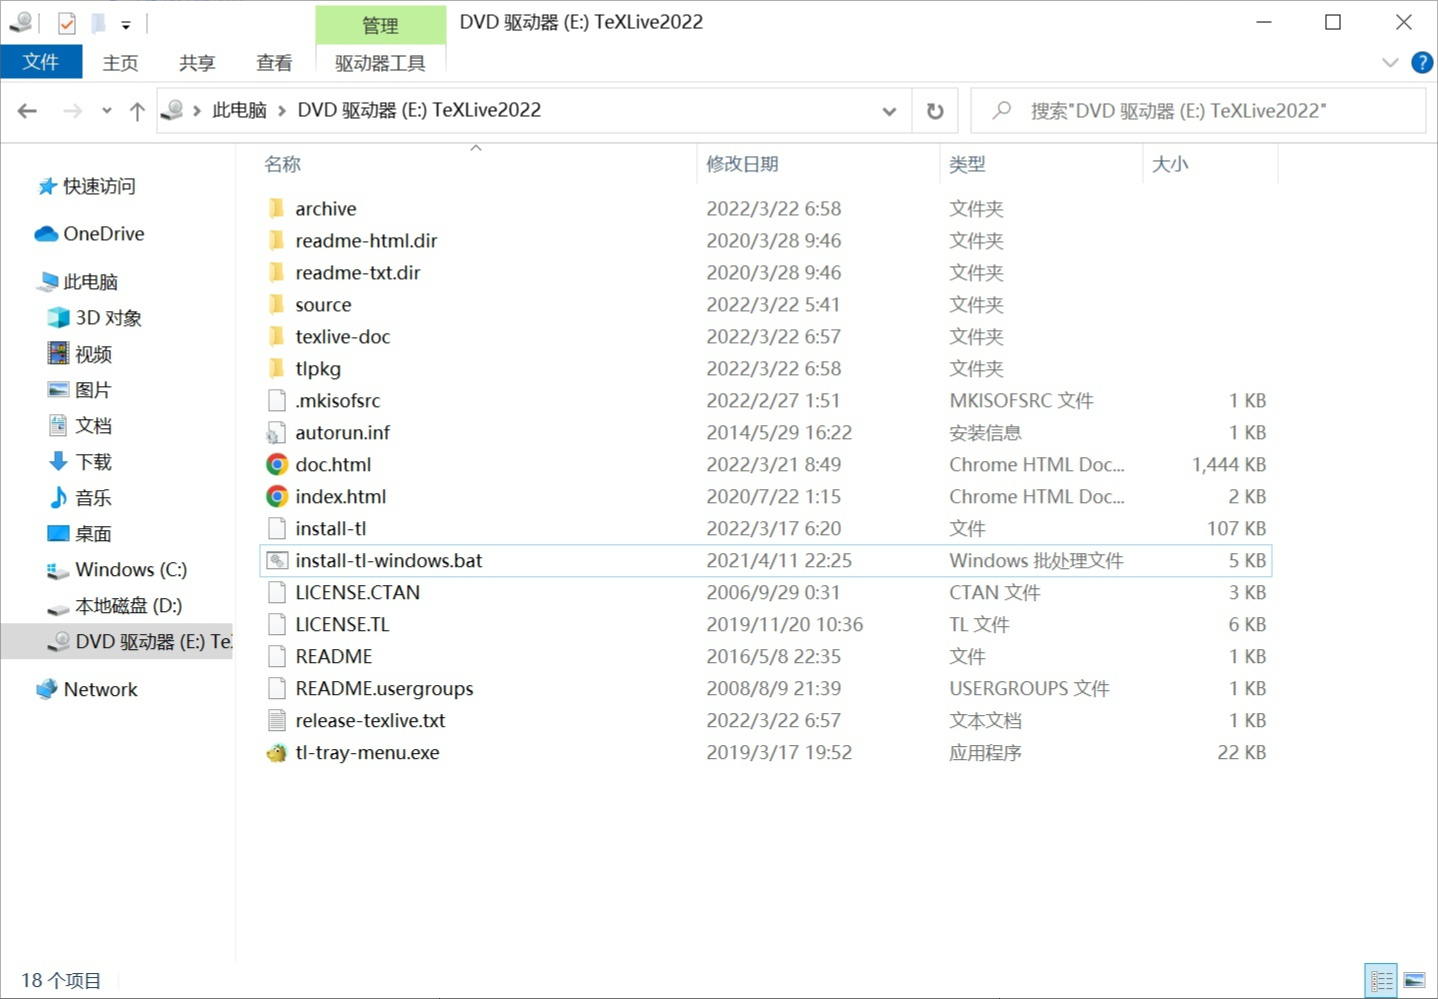
\includegraphics[width=0.95\textwidth]{figures/chapter2/texlive-iso.png}
  \caption{Tex Live镜像}
  \label{fig:2-texlive-iso}
\end{figure}

Windows下直接打开install-tl-windows.bat,Linux/Mac用户在终端下输入:

\begin{lstlisting}[language=bash]
  ./install-tl
\end{lstlisting}

使用默认配置进行安装。

\begin{figure}[htb]
  \centering
  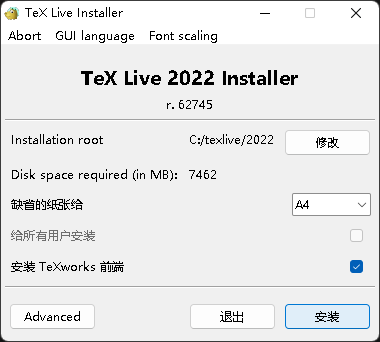
\includegraphics[width=0.4\textwidth]{figures/chapter2/texlive-install.png}
  \caption{Tex Live安装}
  \label{fig:2-texlive-install}
\end{figure}

详细安装过程和注意事项请参考:\url{https://github.com/OsbertWang/install-latex-guide-zh-cn/releases/latest/}

\subsection{VSCode配置}

Tex Live自带的编辑器不太好用,个人一般使用VSCode配合LaTeX Workshop插件。

\begin{enumerate}
  \item 点击拓展图标,打开拓展
  \item 输入"latex workshop",选择第一个LaTeX Workshop插件
  \item 点击"install"进行安装,等待安装完成(如图\ref{fig:2-plugin-install})
\end{enumerate}

\begin{figure}[H]
  \centering
  
\includegraphics[width=0.95\textwidth]{figures/chapter2/plugin-install.png}
  \caption{LaTeX Workshop插件安装}
  \label{fig:2-plugin-install}
\end{figure}

\begin{enumerate}
  \item 点击设置图标
  \item 点击设置
  \item 转到 UI 设置页面(如图\ref{fig:2-vscode-settings})
  \item 点击右上侧图标打开JSON配置文件,进入代码设置页面(如图\ref{fig:2-vscode-json})
\end{enumerate}

\begin{figure}[H]
  \centering
  \begin{subfigure}{0.45\textwidth}
    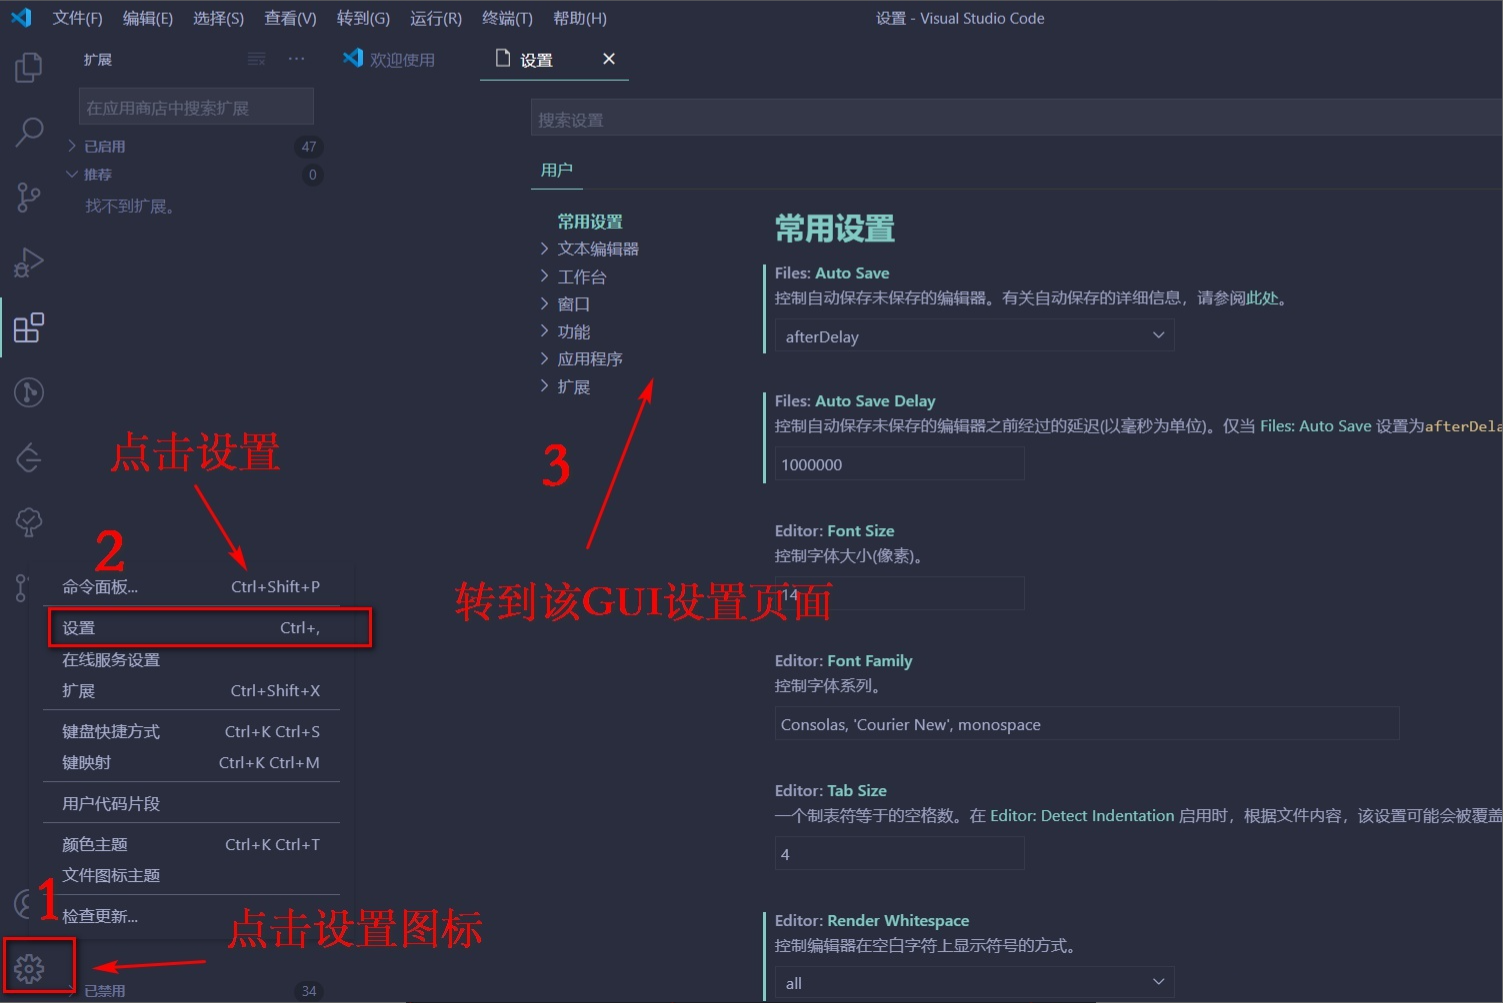
\includegraphics[width=\linewidth]{figures/chapter2/vscode-settings.png}
    \caption{UI设置界面}
    \label{fig:2-vscode-settings}
  \end{subfigure}\qquad
  \begin{subfigure}{0.45\textwidth}
    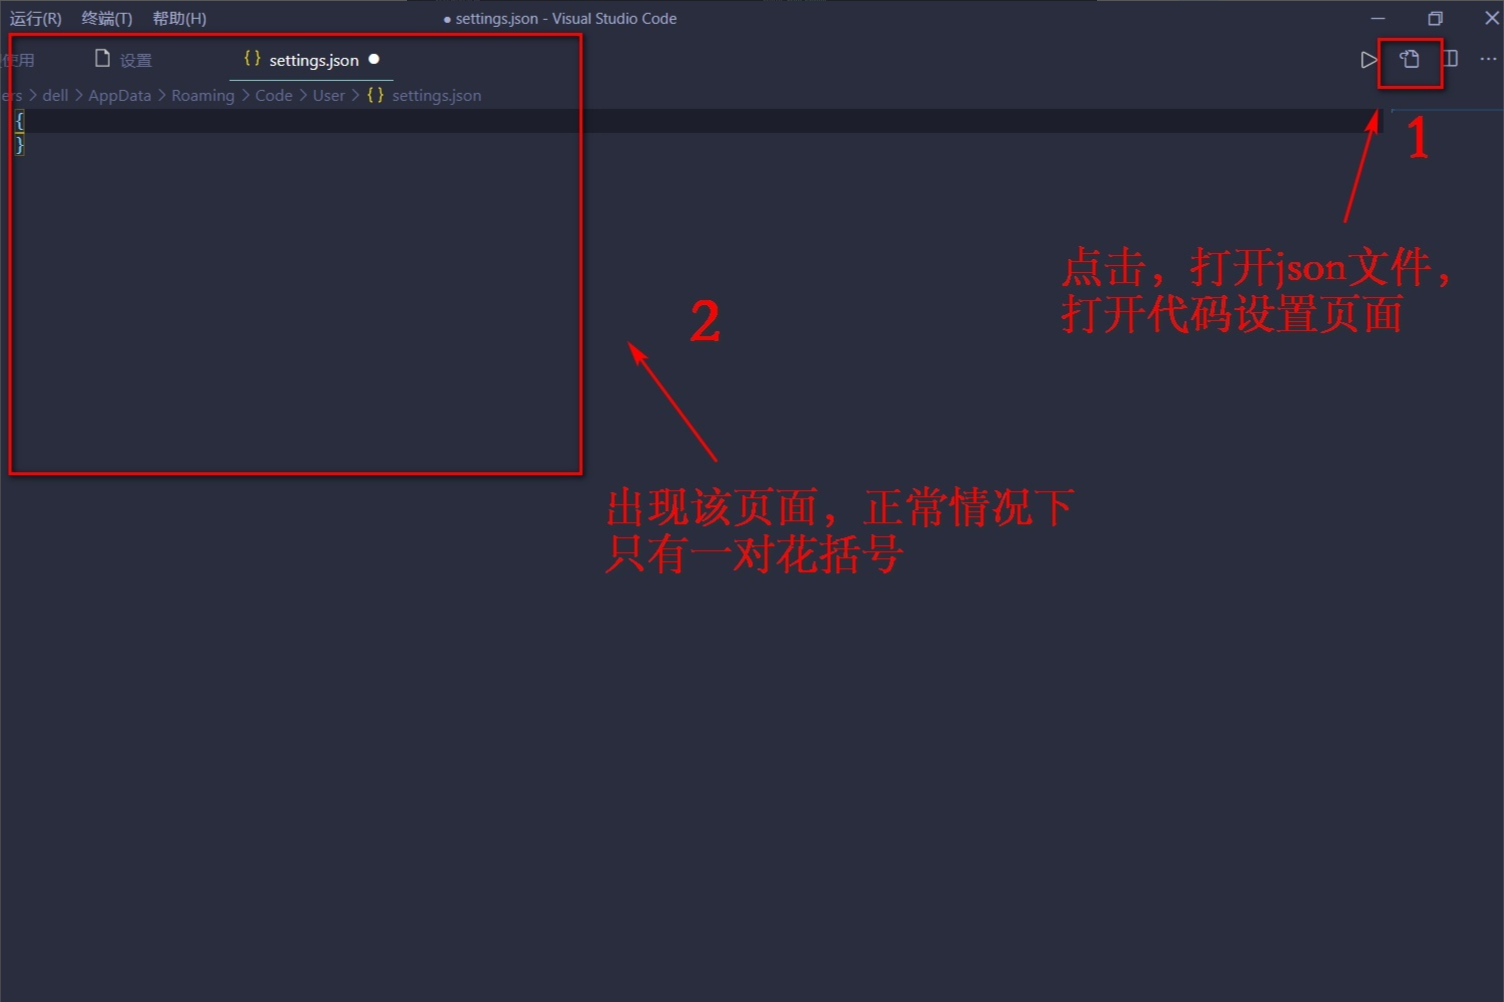
\includegraphics[width=\linewidth]{figures/chapter2/vscode-json.png}
    \caption{JSON配置文件}
    \label{fig:2-vscode-json}
  \end{subfigure}
  \caption{配置~\LaTeX~}
  \label{fig:2-vscode-conf}
\end{figure}

在JSON文件内输入以下内容:

由于PDF内代码不好复制,JSON内容请参考:\url{https://zhuanlan.zhihu.com/p/166523064}\quad \textbf{6.1 LaTeX配置代码展示}处

\begin{lstlisting}[language=json]
  {
    "latex-workshop.latex.autoBuild.run": "never",
    "latex-workshop.showContextMenu": true,
    "latex-workshop.intellisense.package.enabled": true,
    "latex-workshop.message.error.show": false,
    "latex-workshop.message.warning.show": false,
    "latex-workshop.latex.tools": [
        {
            "name": "xelatex",
            "command": "xelatex",
            "args": [
                "-synctex=1",
                "-interaction=nonstopmode",
                "-file-line-error",
                "%DOCFILE%"
            ]
        },
        {
            "name": "pdflatex",
            "command": "pdflatex",
            "args": [
                "-synctex=1",
                "-interaction=nonstopmode",
                "-file-line-error",
                "%DOCFILE%"
            ]
        },
        {
            "name": "latexmk",
            "command": "latexmk",
            "args": [
                "-synctex=1",
                "-interaction=nonstopmode",
                "-file-line-error",
                "-pdf",
                "-outdir=%OUTDIR%",
                "%DOCFILE%"
            ]
        },
        {
            "name": "bibtex",
            "command": "bibtex",
            "args": [
                "%DOCFILE%"
            ]
        }
    ],
    "latex-workshop.latex.recipes": [
        {
            "name": "XeLaTeX",
            "tools": [
                "xelatex"
            ]
        },
        {
            "name": "PDFLaTeX",
            "tools": [
                "pdflatex"
            ]
        },
        {
            "name": "BibTeX",
            "tools": [
                "bibtex"
            ]
        },
        {
            "name": "LaTeXmk",
            "tools": [
                "latexmk"
            ]
        },
        {
            "name": "xelatex -> bibtex -> xelatex*2",
            "tools": [
                "xelatex",
                "bibtex",
                "xelatex",
                "xelatex"
            ]
        },
        {
            "name": "pdflatex -> bibtex -> pdflatex*2",
            "tools": [
                "pdflatex",
                "bibtex",
                "pdflatex",
                "pdflatex"
            ]
        },
    ],
    "latex-workshop.latex.clean.fileTypes": [
        "*.aux",
        "*.bbl",
        "*.blg",
        "*.idx",
        "*.ind",
        "*.lof",
        "*.lot",
        "*.out",
        "*.toc",
        "*.acn",
        "*.acr",
        "*.alg",
        "*.glg",
        "*.glo",
        "*.gls",
        "*.ist",
        "*.fls",
        "*.log",
        "*.fdb_latexmk"
    ],
    "latex-workshop.latex.autoClean.run": "onFailed",
    "latex-workshop.latex.recipe.default": "lastUsed",
    "latex-workshop.view.pdf.internal.synctex.keybinding": "double-click"
}
\end{lstlisting}

\subsection{VSCode编译}

此时你需要将使用的模板下载至本地。以此项目为例,进入\url{https://github.com/Nagico/WHUExperiment},点击Download ZIP即可将模板下载到本地。该模板同时也一同放至本文档旁,可以直接使用,但仍建议从Github上下载最新版本的模板。

\begin{figure}[htb]
  \centering
  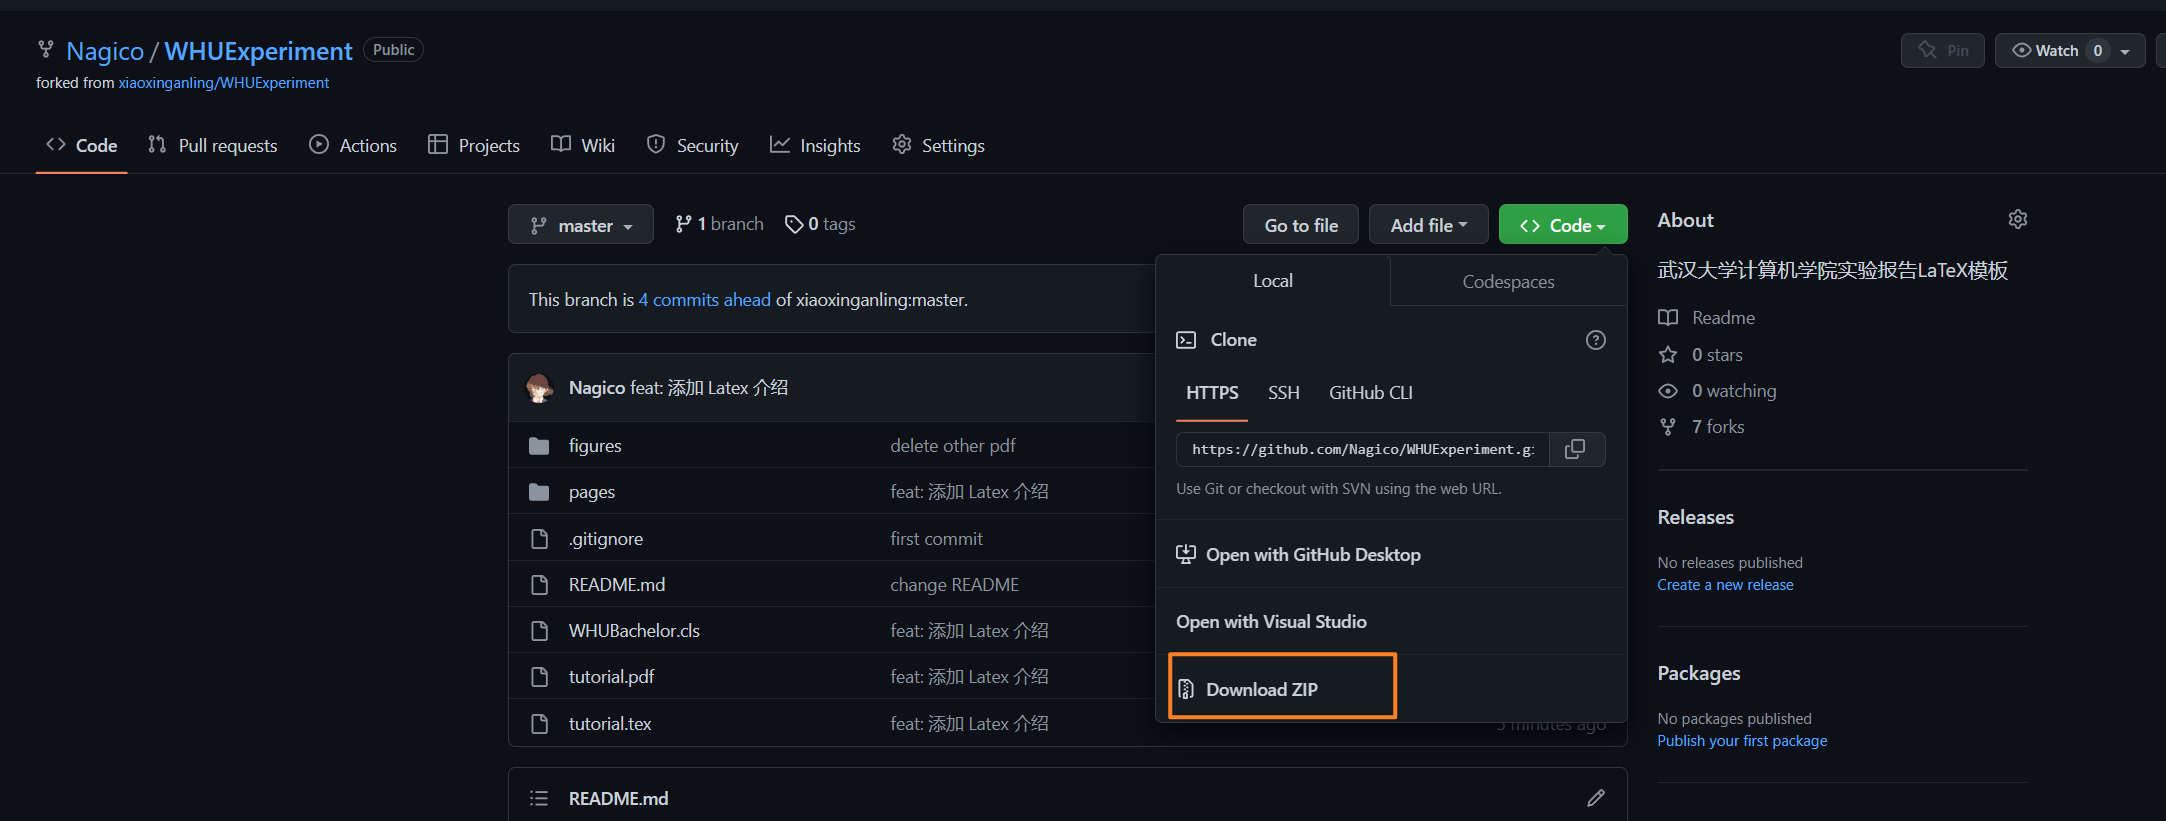
\includegraphics[width=0.95\textwidth]{figures/chapter2/download-repo.png}
  \caption{下载模板}
  \label{fig:2-github-download-2}
\end{figure}

将项目解压后用VSCode打开文件夹,点击选中 tex 文件,进行文件内容查看。

\begin{figure}[H]
  \centering
  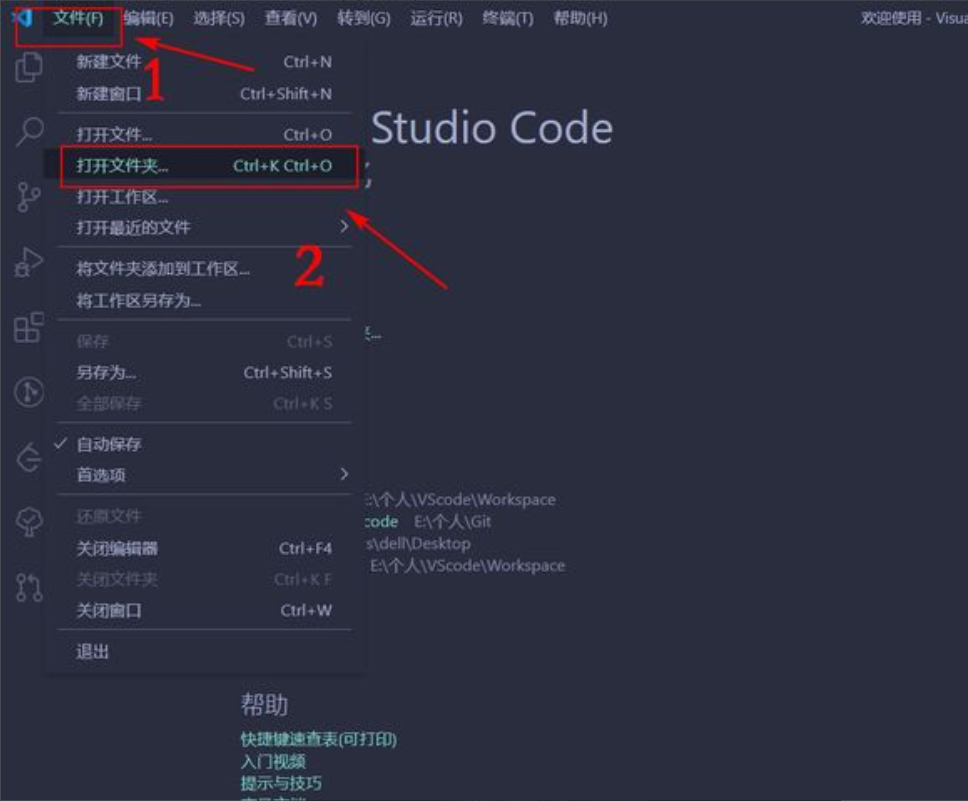
\includegraphics[width=0.9\textwidth]{figures/chapter2/vscode-open.png}
  \caption{打开项目文件夹}
  \label{fig:2-vscode-open-folder}
\end{figure}

\begin{figure}[H]
  \centering
  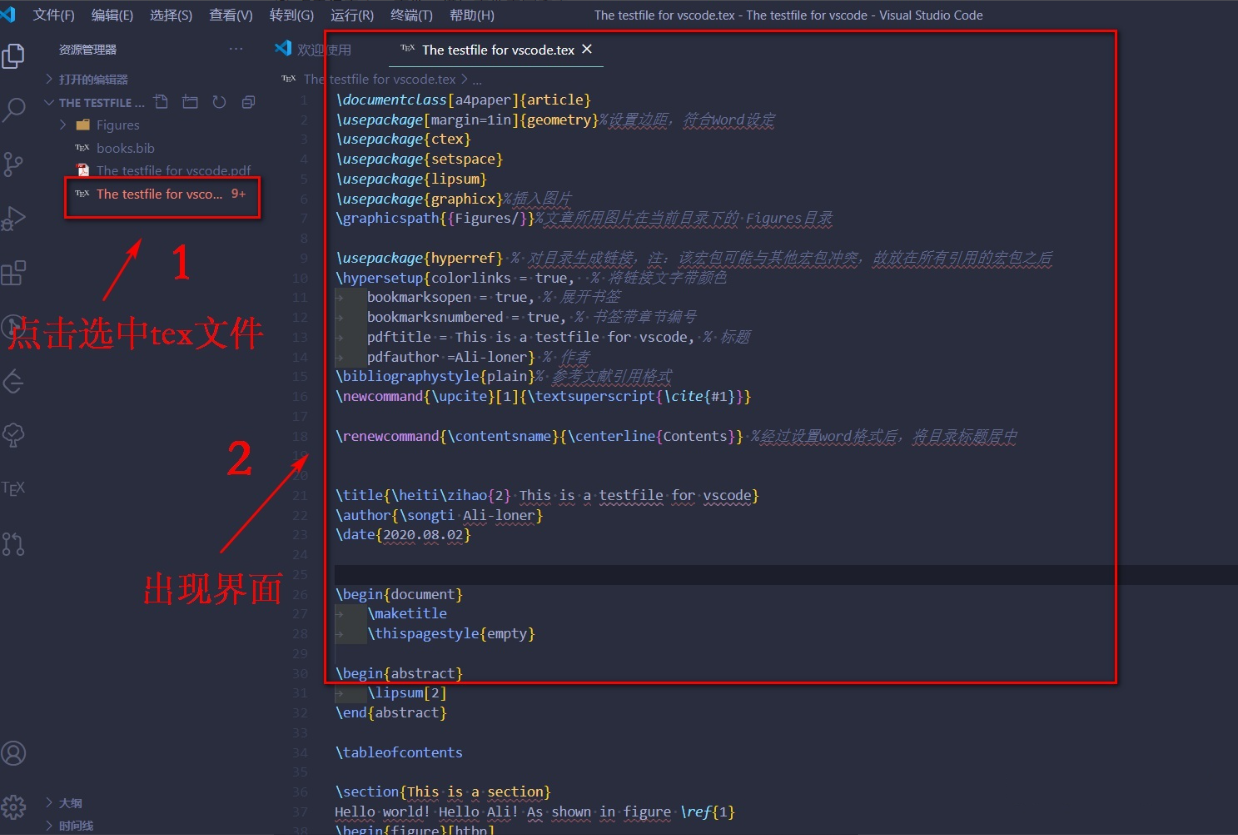
\includegraphics[width=0.9\textwidth]{figures/chapter2/vscode-openfile.png}
  \caption{打开Tex文件}
  \label{fig:2-vscode-open-file}
\end{figure}

由于项目中会涉及参考文献的引用(.bib的编译),故而选择xelatex -> bibtex -> xelatex*2编译链。

\begin{figure}[htb]
  \centering
  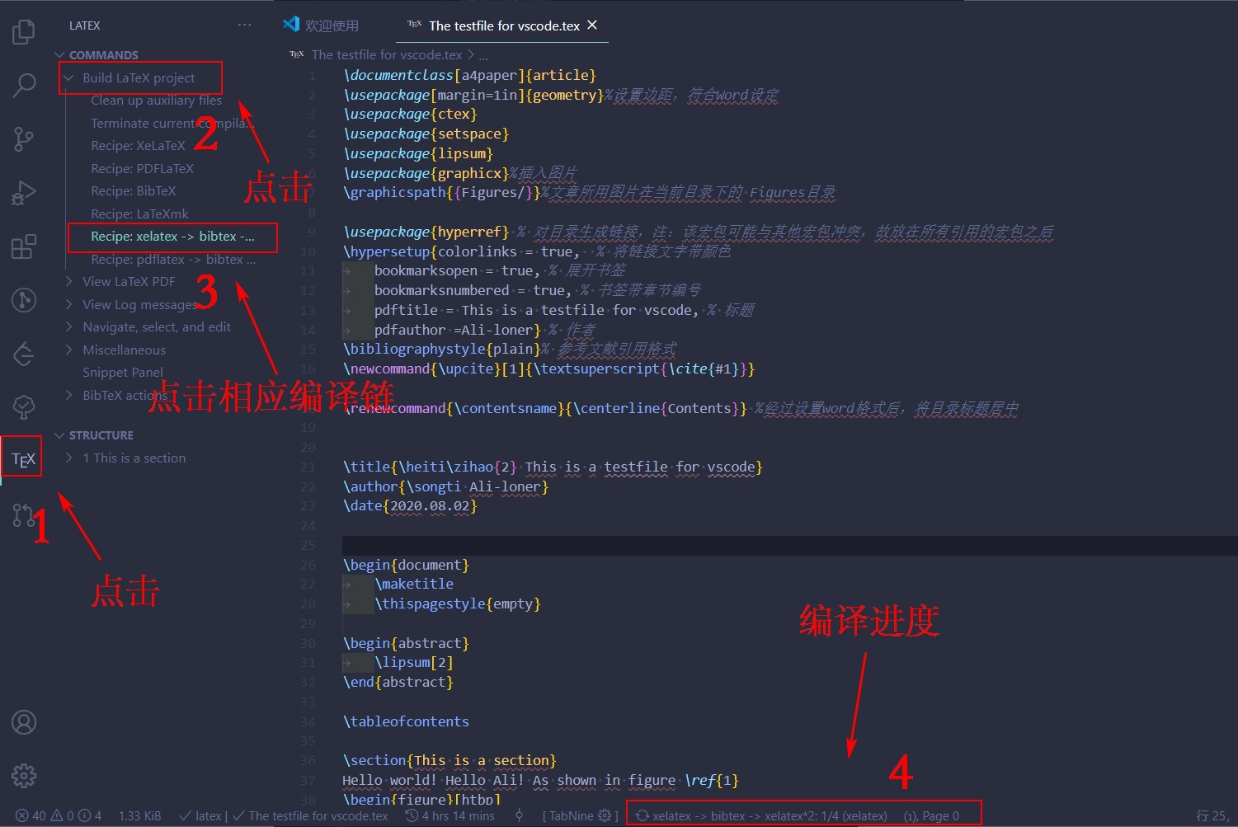
\includegraphics[width=0.8\textwidth]{figures/chapter2/vscode-compile.png}
  \caption{Tex编译}
  \label{fig:2-vscode-tex-compile}
\end{figure}

点击编辑界面的右上角图标,即可查看编译结果。

\begin{figure}[H]
  \centering
  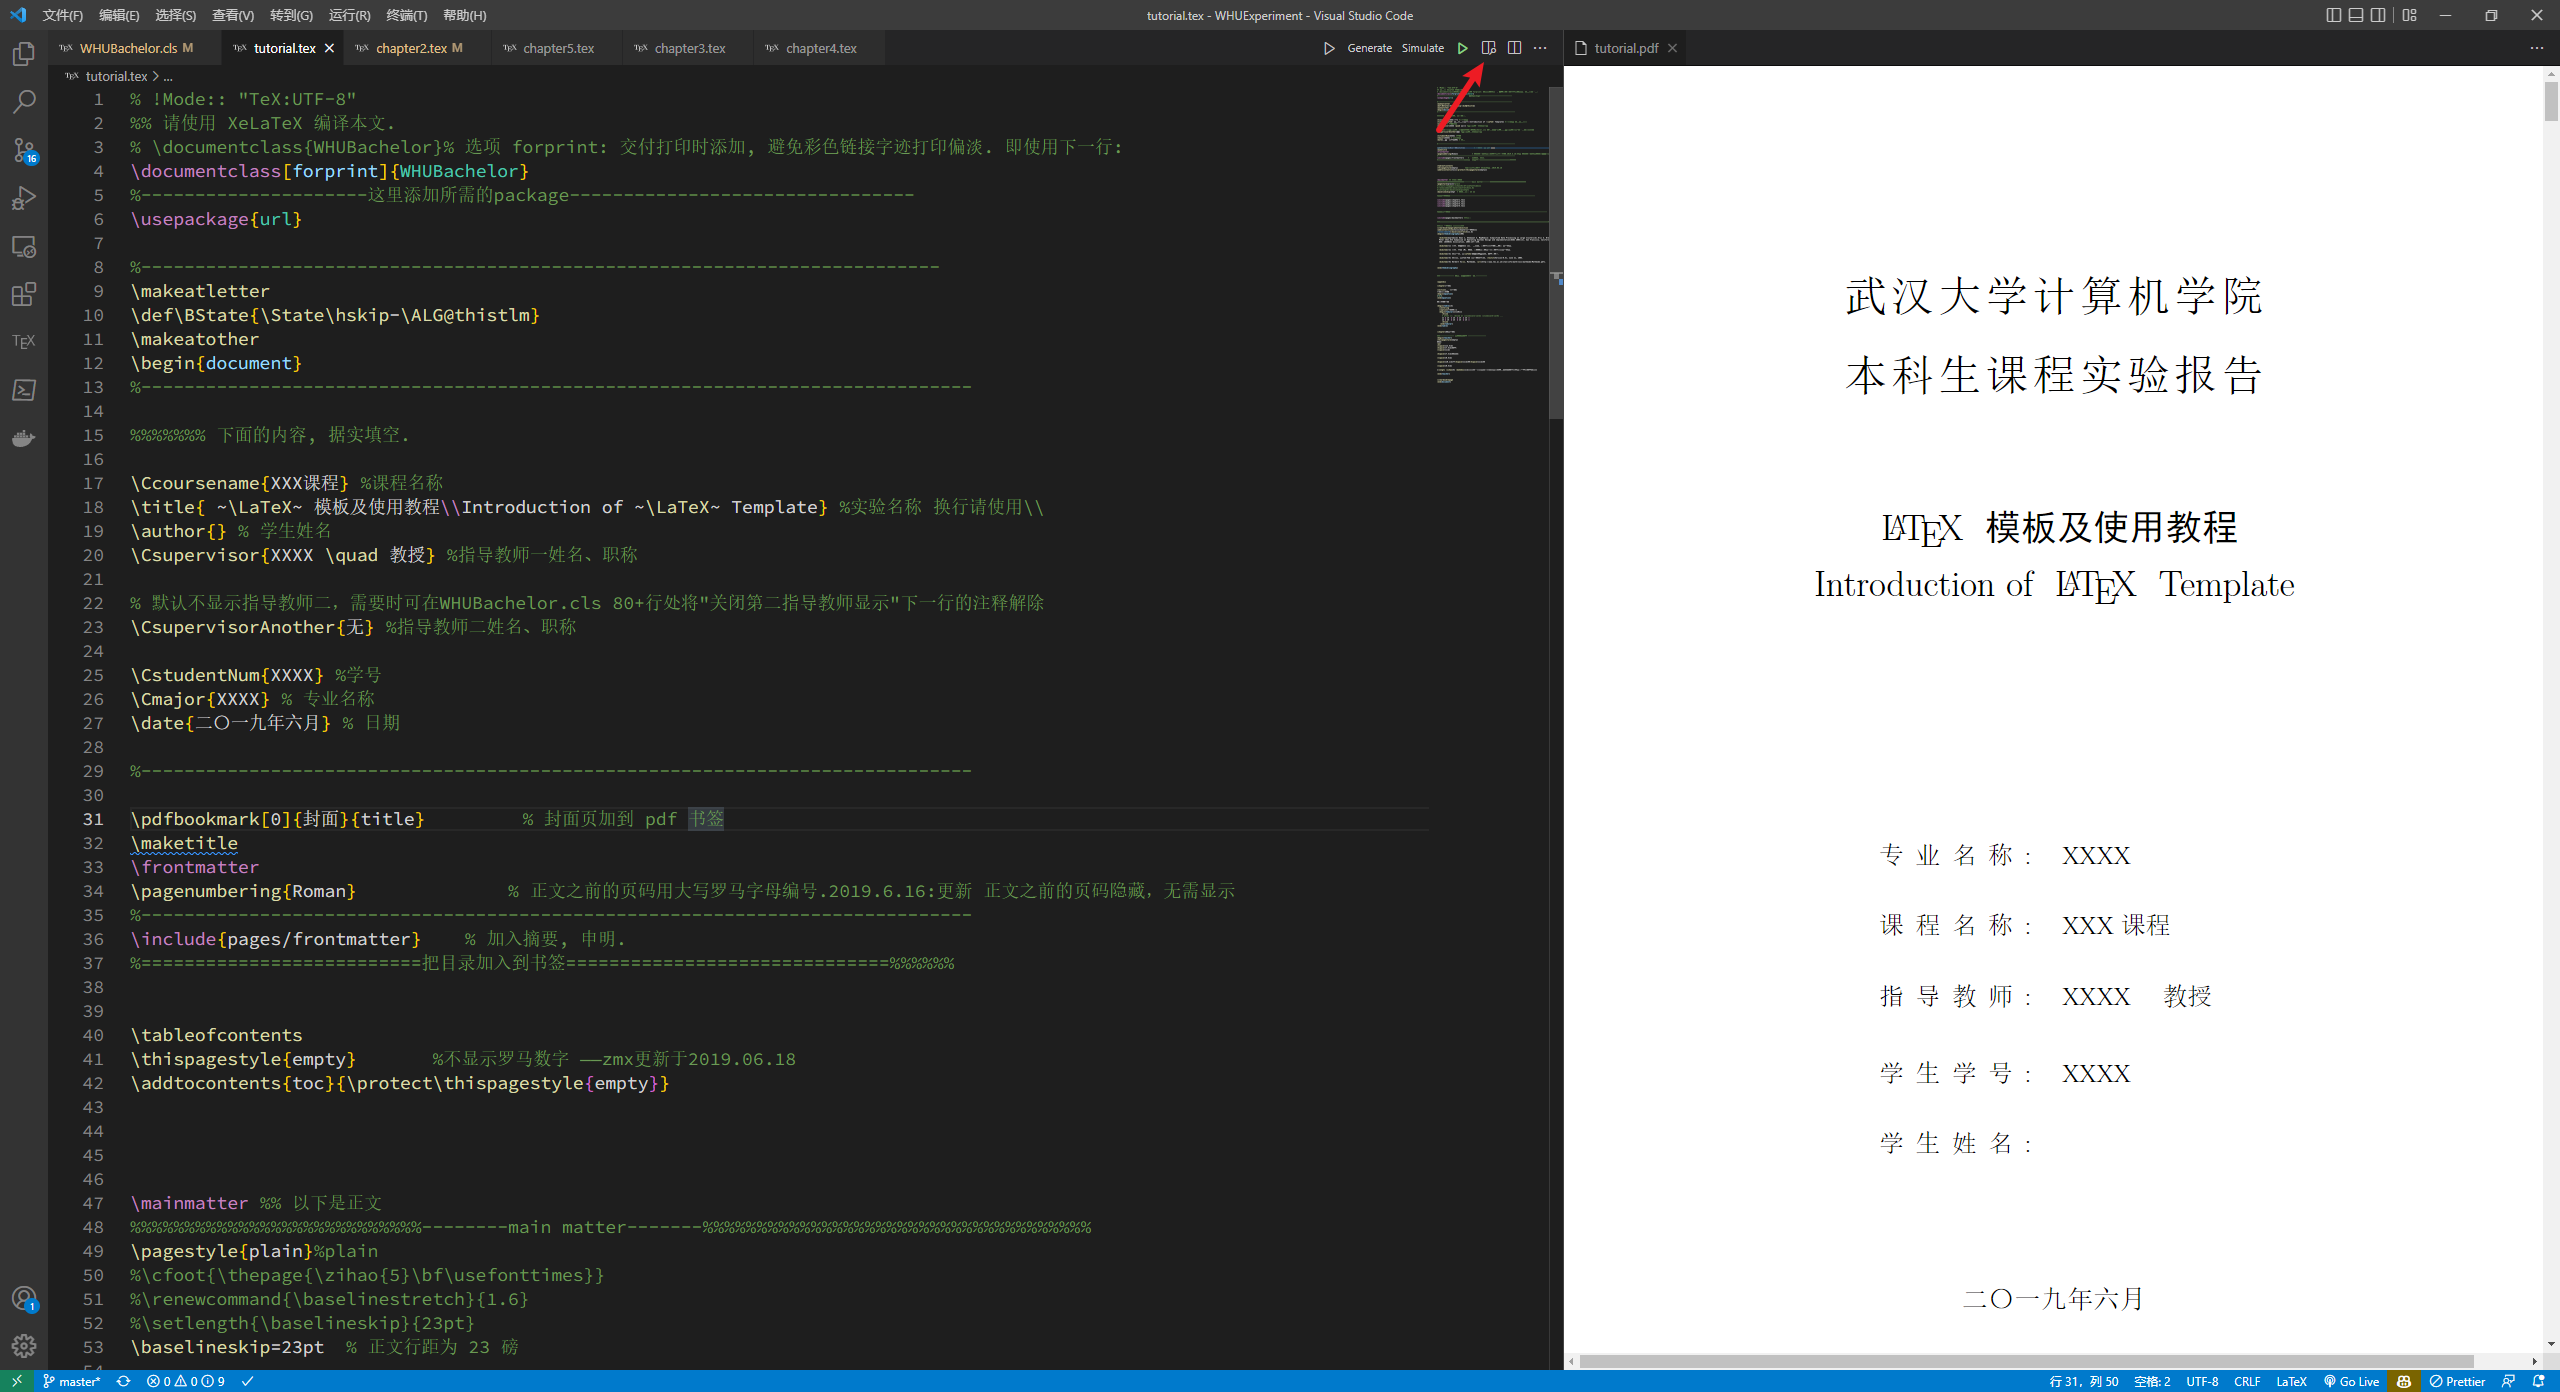
\includegraphics[width=0.95\textwidth]{figures/chapter2/vscode-edit.png}
  \caption{Tex编译结果}
  \label{fig:2-vscode-edit}
\end{figure}

更多VSCode配置可参考网上Blog,实现双向自动跳转等功能。新版VSCode、插件与以前有一定差别,最好选择2022年及以后较新的Blog学习。
\chapter{模板使用教程}
 
\section{Readme}

模板文件的结构, 如下表所示:
 \begin{table}[ht]\centering
\begin{tabular}{r|r|l}
	\hline\hline
	\multicolumn{2}{l|}{main.tex }       & 主文档. 在其中填写首页信息、正文引用、参考文献引用。             \\ \hline
                                    & chapter$x$.tex & 第$x$章节正文。             \\ \cline{2-3}
    \raisebox{1em}{pages 文件夹}   & frontmatter.tex & 郑重声明、摘要。               \\ \cline{2-3}
	 &  backmatter.tex & 实验结论.                       \\ \hline
	\multicolumn{2}{l|}{figures 文件夹}                  & 存放图片文件。                   \\ \hline
    \multicolumn{2}{l|}{ref 文件夹}                  & 存放Bib参考文献文件。                   \\ \hline
	\multicolumn{2}{l|}{WHUBachelor.cls }             & 定义文档格式的 class file。不可删除。 \\ \hline\hline
\end{tabular}
\end{table}

无需也不要改变、移动上述文档的位置。

如果不习惯用~\verb|\include{ }|~的方式加入“子文档”,当然可以把它们合并在主文档,成为一个文档。
({\kaishu 但是这样并不会给我们带来方便。})

 \section{具体使用步骤}

 \begin{description}
  \item[Step 1]  打开主文档 main.tex,填写题目、学生姓名等等信息,书写正文。
  \item[Step 2]  进入 pages 文件夹,打开 frontmatter.tex,backmatter.tex 这两个文档,
  分别填写 (1) 中文摘要,(2) 实验结论。并根据实际情况创建chapter tex文件书写正文。
  \item[Step 3]  打开主文档,在正文部分修改include的文件,注意此时不需要tex后缀名。
  \item[Step 4]  导入bib参考文献,在文档中引用。 
  \item[Step 5]  使用 XeLaTeX 编译。
\end{description}

\section{其他}

自此,~\LaTeX~安装与模板使用说明已介绍完毕。接下来的章节会以本模板支持的命令为例,讲解~\LaTeX~的使用方法。请将PDF配合Tex源码一同学习,可自行修改相关命令,查看效果。

其中 Chapter \ref{cha:latex-brief-intro}将简要的介绍~\LaTeX~使用方法,包括多级标题、字体样式、字号调节、定理与公式、图片与表格的简单使用。初次学习可以参考此章节。


 \vfill

本文档下载更新地址:\url{https://github.com/Nagico/WHUExperiment}. 使用之前,请移步查看是否有更新。
\chapter{杂七杂八的话}

\section{Readme}

模板文件的结构, 如下表所示:
 \begin{table}[ht]\centering
\begin{tabular}{r|r|l}
	\hline\hline
	\multicolumn{2}{l|}{Experiment-template.tex }       & 主文档. 在其中填写正文.             \\ \hline
	                                & frontmatter.tex & 郑重声明、摘要.               \\ \cline{2-3}
	\raisebox{1em}{includefile 文件夹} &  backmatter.tex & 实验结论.                       \\ \hline
	\multicolumn{2}{l|}{figures 文件夹}                  & 存放图片文件.                   \\ \hline
	\multicolumn{2}{l|}{WHUBachelor.cls }             & 定义文档格式的 class file. 不可删除. \\ \hline\hline
\end{tabular}
\end{table}

无需也不要改变、移动上述文档的位置.

如果不习惯用~\verb|\include{ }|~的方式加入``子文档'', 当然可以把它们合并在主文档, 成为一个文档.
({\kaishu 但是这样并不会给我们带来方便.})




 \section{字体调节}

\begin{tabular}{ll}
	\verb|\songti|   & {\songti 宋体}   \\
	\verb|\heiti|    & {\heiti 黑体}    \\
	\verb|\fangsong| & {\fangsong 仿宋} \\
	\verb|\kaishu|   & {\kaishu 楷书}
\end{tabular}


\section{字号调节}
字号命令: \verb|\zihao| \index{zihao}

\begin{tabular}{ll}
\verb|\zihao{0}| &\zihao{0}  初号字 English \\
\verb|\zihao{-0}|&\zihao{-0} 小初号 English \\
\verb|\zihao{1} |&\zihao{1}  一号字 English \\
\verb|\zihao{-1}|&\zihao{-1} 小一号 English \\
\verb|\zihao{2} |&\zihao{2}  二号字 English \\
\verb|\zihao{-2}|&\zihao{-2} 小二号 English \\
\verb|\zihao{3} |&\zihao{3}  三号字 English \\
\verb|\zihao{-3}|&\zihao{-3} 小三号 English \\
\verb|\zihao{4} |&\zihao{4}  四号字 English \\
\verb|\zihao{-4}|&\zihao{-4} 小四号 English \\
\verb|\zihao{5} |&\zihao{5}  五号字 English \\
\verb|\zihao{-5}|&\zihao{-5} 小五号 English \\
\verb|\zihao{6} |&\zihao{6}  六号字 English \\
\verb|\zihao{-6}|&\zihao{-6} 小六号 English \\
\verb|\zihao{7} |&\zihao{7}  七号字 English \\
\verb|\zihao{8} |&\zihao{8}  八号字 English \\
\end{tabular}

\section{已加入的常用宏包}

\begin{description}
%  \item[amsmath,amssymb]
  \item[cite]  参考文献引用, 得到形如 [3-7] 的样式.
  \item[color,xcolor]  支持彩色.
  \item[enumerate]  方便自由选择 enumerate 环境的编号方式. 比如

  \verb|\begin{enumerate}[(a)]| 得到形如 (a), (b), (c) 的编号.


  \verb|\begin{enumerate}[i)]| 得到形如 i), ii), iii) 的编号.

  \verb|\begin{enumerate}[\hspace{1cm}(1)]| \verb|\hspace|命令用于调整距离

\end{description}

另外要说明的是,  itemize, enumerate, description 这三种 list 环境, 已经调节了其间距和缩进,
以符合中文书写的习惯.

\section{标点符号的问题}

建议使用半角的标点符号, 后边再键入一个空格. 特别是在英文书写中要注意此问题!

双引号是由两个左单引号、两个右单引号构成的: \verb|``  ''|. 左单引号在键盘上数字~1 的左边.

但是, 无论您偏向于全角或半角, 强烈建议您使用实心的句号, 只要您书写的是自然科学的文章.
原因可能是因为, 比如使用全角句号的句子结尾处的``$x$。''容易误为数学式~$x_0$(\verb|$x_0$|)吧.



\section{引用的问题}


\subsection{参考文献的引用}

参考文献的引用, 用命令~\verb|\cite{ }|. 大括号内要填入的字串, 是自命名的文献条目名.

比如, 通常我们会说:

 {\kaishu
关于此问题, 请参见文献 \cite{r2}. 作者某某还提到了某某概念\upcite{r1}.}


上文使用的源文件为:

 {\kaishu
关于此问题, 请参见文献~\verb|\cite{r2}|. 作者某某还提到了某某概念~\verb|\upcite{r1}|.
}

其中~\verb|\upcite| 是自定义命令, 使文献引用呈现为\CJKunderdot{上标形式}.

({\heiti 注意:} {\kaishu 这里文献的引用, 有时需要以上标形式出现, 有时需要作为正文文字出现, 为什么?})

另外, 要得到形如~\cite{r1,r3,r4,r5} 的参考文献连续引用, 需要用到 cite 宏包(模板已经加入),
在正文中使用~\verb|\cite{r1,r3,r4,r5}| 的引用形式即可.
或者, 连续引用的上标形式: 使用~\verb|\upcite{r1,r2,r3}|, 得到\upcite{r1,r2,r3}.

\subsection{定理和公式的引用}

\begin{theorem}[谁发现的]\label{th-abcd}
最大的正整数是~$1$.
\end{theorem}

\begin{proof}
要找到这个最大的正整数, 我们设最大的正整数为~$x$, 则~$x \geqslant 1$, 两边同时乘以~$x$, 得到
\begin{equation}\label{eq-abc}
x^2 \geqslant x.
\end{equation}
而~$x$ 是最大的正整数, 由~\eqref{eq-abc} 式得到
\[
x^2 = x.
\]
所以
\begin{equation*}
x = 1.
\end{equation*}
\end{proof}

定理~\ref{th-abcd} 是一个重大的发现.

%%%%----- 定义等环境的举例 --------
\begin{definition}[整数]
 正整数(例如 1, 2, 3)、负整数(例如 ${−1}$, $−2$, $−3$)与零(0)合起来统称为{\heiti 整数}.
\end{definition}

\begin{remark}
  整数集合在数学上通常表示为 $\mathbf{Z}$ 或 $\mathbb{Z}$, 该记号源于德语单词 Zahlen(意为``数'')的首字母.
\end{remark}

\begin{proposition}
任意两个整数相加、相减、相乘的结果, 仍然是整数.
\end{proposition}

\begin{example}
  $1+2=3$.
\end{example}

\begin{corollary}
   在整数集合内, 相加、相减、相乘运算是封闭的.
\end{corollary}

\section{图形与表格}

支持对~eps, pdf, jpg 等等常见图形格式.

再次\colorbox{red!45}{澄清一个误会}: \LaTeX{} 支持的图形格式绝非 eps 这一种. 无需特意把图片转化为 eps.

用形如~\verb|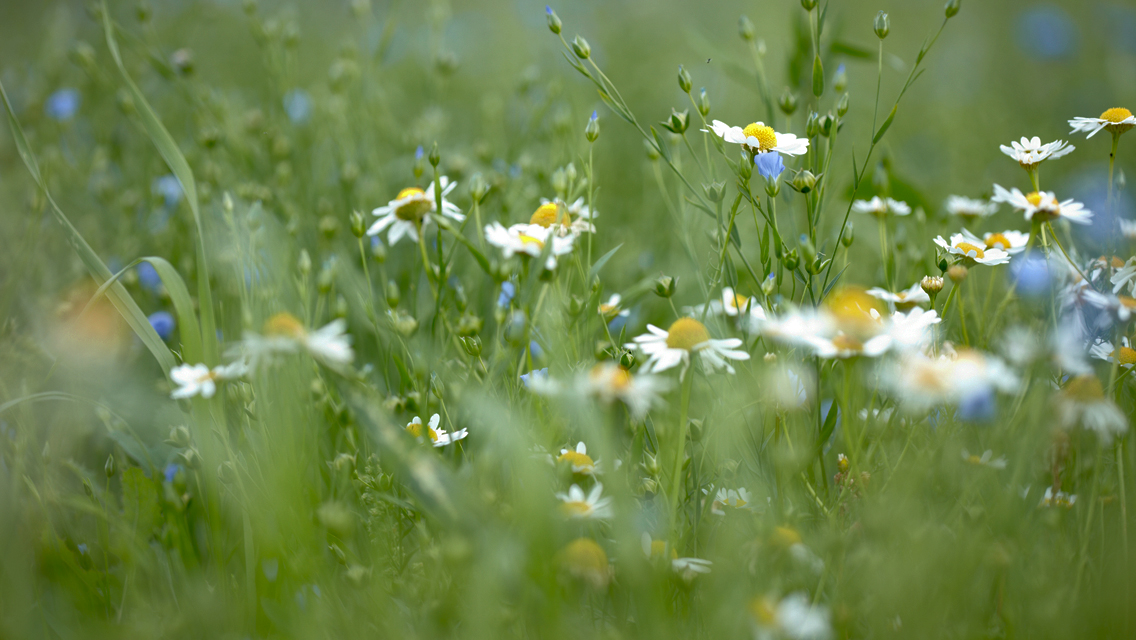
\includegraphics[width=12cm]{Daisy.jpg}| 的命令可以纳入图片.

如图~\ref{fig:1} 是一个纳入~jpg 图片的例子.

\begin{figure}[ht]
\centering
  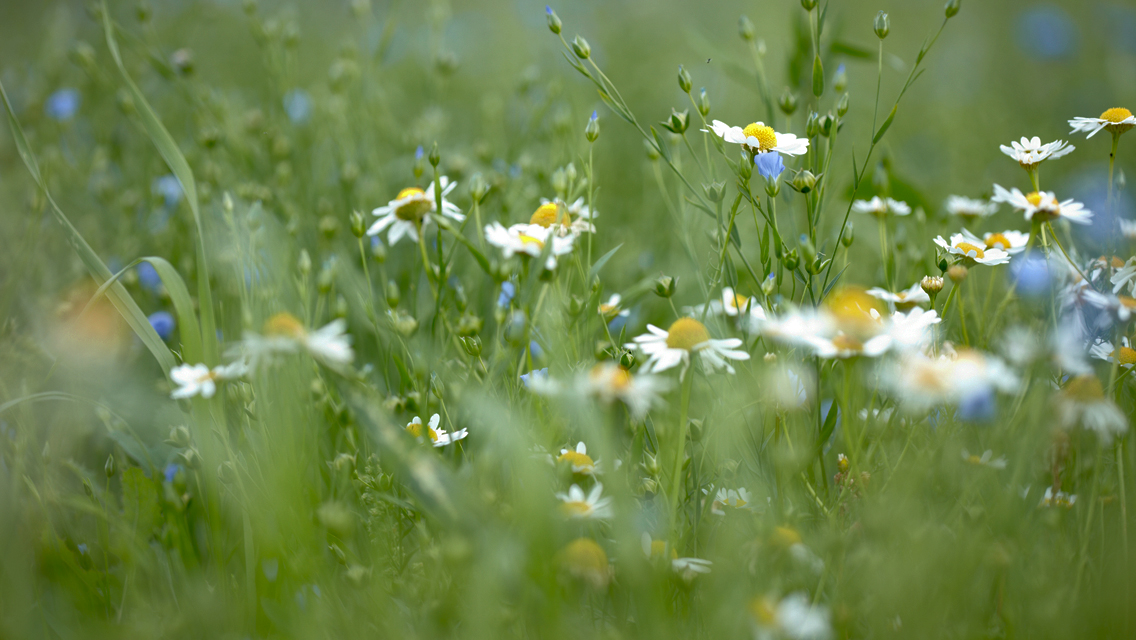
\includegraphics[width=\textwidth]{Daisy.jpg}
  \caption{一个彩色 jpg 图片的例子}
  \label{fig:1}
\end{figure}

表格问题, 建议使用``三线表'', 如表 \ref{tab:1}.

\begin{table}[ht]
\centering
\caption{一般三线表}
\label{tab:1}
    \begin{tabular}{c c c c c c c c c c c}
    \hline
    123 & 4  & 5  & 123 & 4 & 5123 & 4 & 5 & 123 & 4 & 5\\
    \hline
    67 & 890 & 13 & 123 & 4 & 5123 & 4 & 5 & 123 & 4 & 5\\
    67 & 890 & 13 & 123 & 4 & 5123 & 4 & 5 & 123 & 4 & 5\\
    67 & 890 & 13 & 123 & 4 & 5123 & 4 & 5 & 123 & 4 & 5\\
    \hline
    \end{tabular}
\end{table}


%%%%============================================================================================================%%%


%此处结束正文-------------------------------------------------------------------------------------------------


% !Mode:: "TeX:UTF-8"
%%%%%%%%%%%%%%%%%%%%%%%%%%%%-------结论--------%%%%%%%%%%%%%%%%%%%%%%%%%%%%%%%%

\acknowledgement
\addcontentsline{toc}{chapter}{结论}
%\linespread{1.5}

这里写本次实验的结论。

% 这里写本次实验的结论
















 %%%结论

%%%============================================================================================================%%%

%%%=== 参考文献 ========%%%
\cleardoublepage\phantomsection
\addcontentsline{toc}{chapter}{参考文献}
\renewcommand{\baselinestretch}{1.6}
\begin{thebibliography}{00}

  \bibitem{mapreduce} Dean J, Ghemawat S. MapReduce: Simplified Data Processing on Large Clusters[A].Eric A. Brewer, Peter Chen.6th Symposium on Operating Systems Design and Implementation(OSDI 2004)[C], San Francisco, California, USA: {USENIX} Association, 2004:137--150.

  \bibitem{r1} 作者. 文章题目 [J].  期刊名, 出版年份,卷号(期数): 起止页码.

  \bibitem{r2} 作者. 书名 [M]. 版次. 出版地:出版单位,出版年份:起止页码.

  \bibitem{r3} 邓建松等, 《\LaTeXe~科技排版指南》, 科学出版社.

  \bibitem{r4} 吴凌云, 《CTeX~FAQ (常见问题集)》, \textit{Version~0.4}, June 21, 2004.

  \bibitem{r5} Herbert Vo\ss, Mathmode, \url{http://www.tex.ac.uk/ctan/info/math/voss/mathmode/Mathmode.pdf}.


\end{thebibliography}



%%%-------------- 附录. 不需要可以删除.-----------


\appendix

\chapter{测试}

\section{第一个测试}
测试公式编号
\begin{equation}
1+1=2.
\end{equation}

表格编号测试

\begin{table}[h]
  \centering
  \caption{测试表格}
  \begin{tabular}{*{20}c}
     \hline
     % after \\: \hline or \cline{col1-col2} \cline{col3-col4} ...
     11 & 13  & 13  & 13  & 13 \\
     12 & 14  & 13  & 13  & 13 \\
     \hline
   \end{tabular}
\end{table}


\chapter{附录测试}

%%%-------------- 教师评语评分 ------------------
\begin{teacher}
\thispagestyle{empty}
评语: 
\par
\vspace*{12.5cm}
\hspace*{7.5cm}评分: 
\vspace*{1cm}

\hspace*{7.3cm}评阅人:

\vspace*{0.5cm}

\hspace*{10.1cm}年\hspace*{1cm}月\hspace*{1cm}日

\vspace*{0.5cm}

{\songti \zihao{4} \makebox[1cm][s]{(备注:对该实验报告给予优点和不足的评价,并给出百分制评分。)}}

\end{teacher}


\cleardoublepage
\end{document}





